\qrchapter{https://forgottenpillar.com/rsc/hr-fp-chapter23}{Veliki otpad uskoro će se ostvariti} \label{chap:apostasy}

Godine 1903., kada je Živi Hram bio objavljen i izazvao kontroverzu oko \emcap{ličnosti Boga}, sestra White je vjerno slušala zapovijed Velikog Zapovjednika. Bila je pozvana riječima “\textit{Suoči se!}” Suočila se s tom kontroverzom pišući brojna pisma mnogim ljudima na polju rada. U tim pismima imamo proročki uvid u budućnost Crkve Adventista Sedmoga Dana.

Jedan primjer je prepiska između sestre White i njezina sina Williama Whitea. Dana 26. studenog 1905. održana je velika Konferencija o zdravlju u College Viewu, Nebraska, gdje su se okupili mnogi medicinski misionari. William White je bio tamo i imao je kratki, 30-minutni javni govor. Nakon toga, napisao je pismo svojoj majci u vezi sa svojim dojmovima s konferencije. Evo dijela tog pisma:

\others{College View, Ne. – utorak, 28. studenog 1905.; Autor: William C. White} \\
\others{28. studenog 1905.} \\
\others{Gospođa E. G. White, Sanatorij, Kalifornija}

\othersnogap{...Subotom ujutro imao sam priliku govoriti trideset minuta. U svojim napomenama referirao sam na povijest kršćanske crkve. Započeli su s čistim principima, ali kroz Sotonine napade otpali su i odstupili su od tih principa. \textbf{Istaknuo sam da je jedina nada za crkvu Adventista Sedmoga Dana \underline{prionuti uz prve principe}}. \textbf{Tada sam se referirao na redoslijed kojim neprijatelj napada naš rad. Njegov prvi pokušaj bio je uništiti jedinstvo i uspostaviti razdvajanje. Njegov sljedeći posao bio je oslabiti naše poštovanje prema suboti, a zatim oslabiti našu vjeru u službu u Svetištu, zatim \underline{uništiti naše pouzdanje u Duh Proroštva}, zatim \underline{zbuniti našu koncepciju o osobnom Bogu}}.}[Letter from W. C. White to E. G. White, November 28, 1905.][http://ellenwhite.org/content/correspondence/incoming/43292pdf]

\begin{figure}
    \centering
    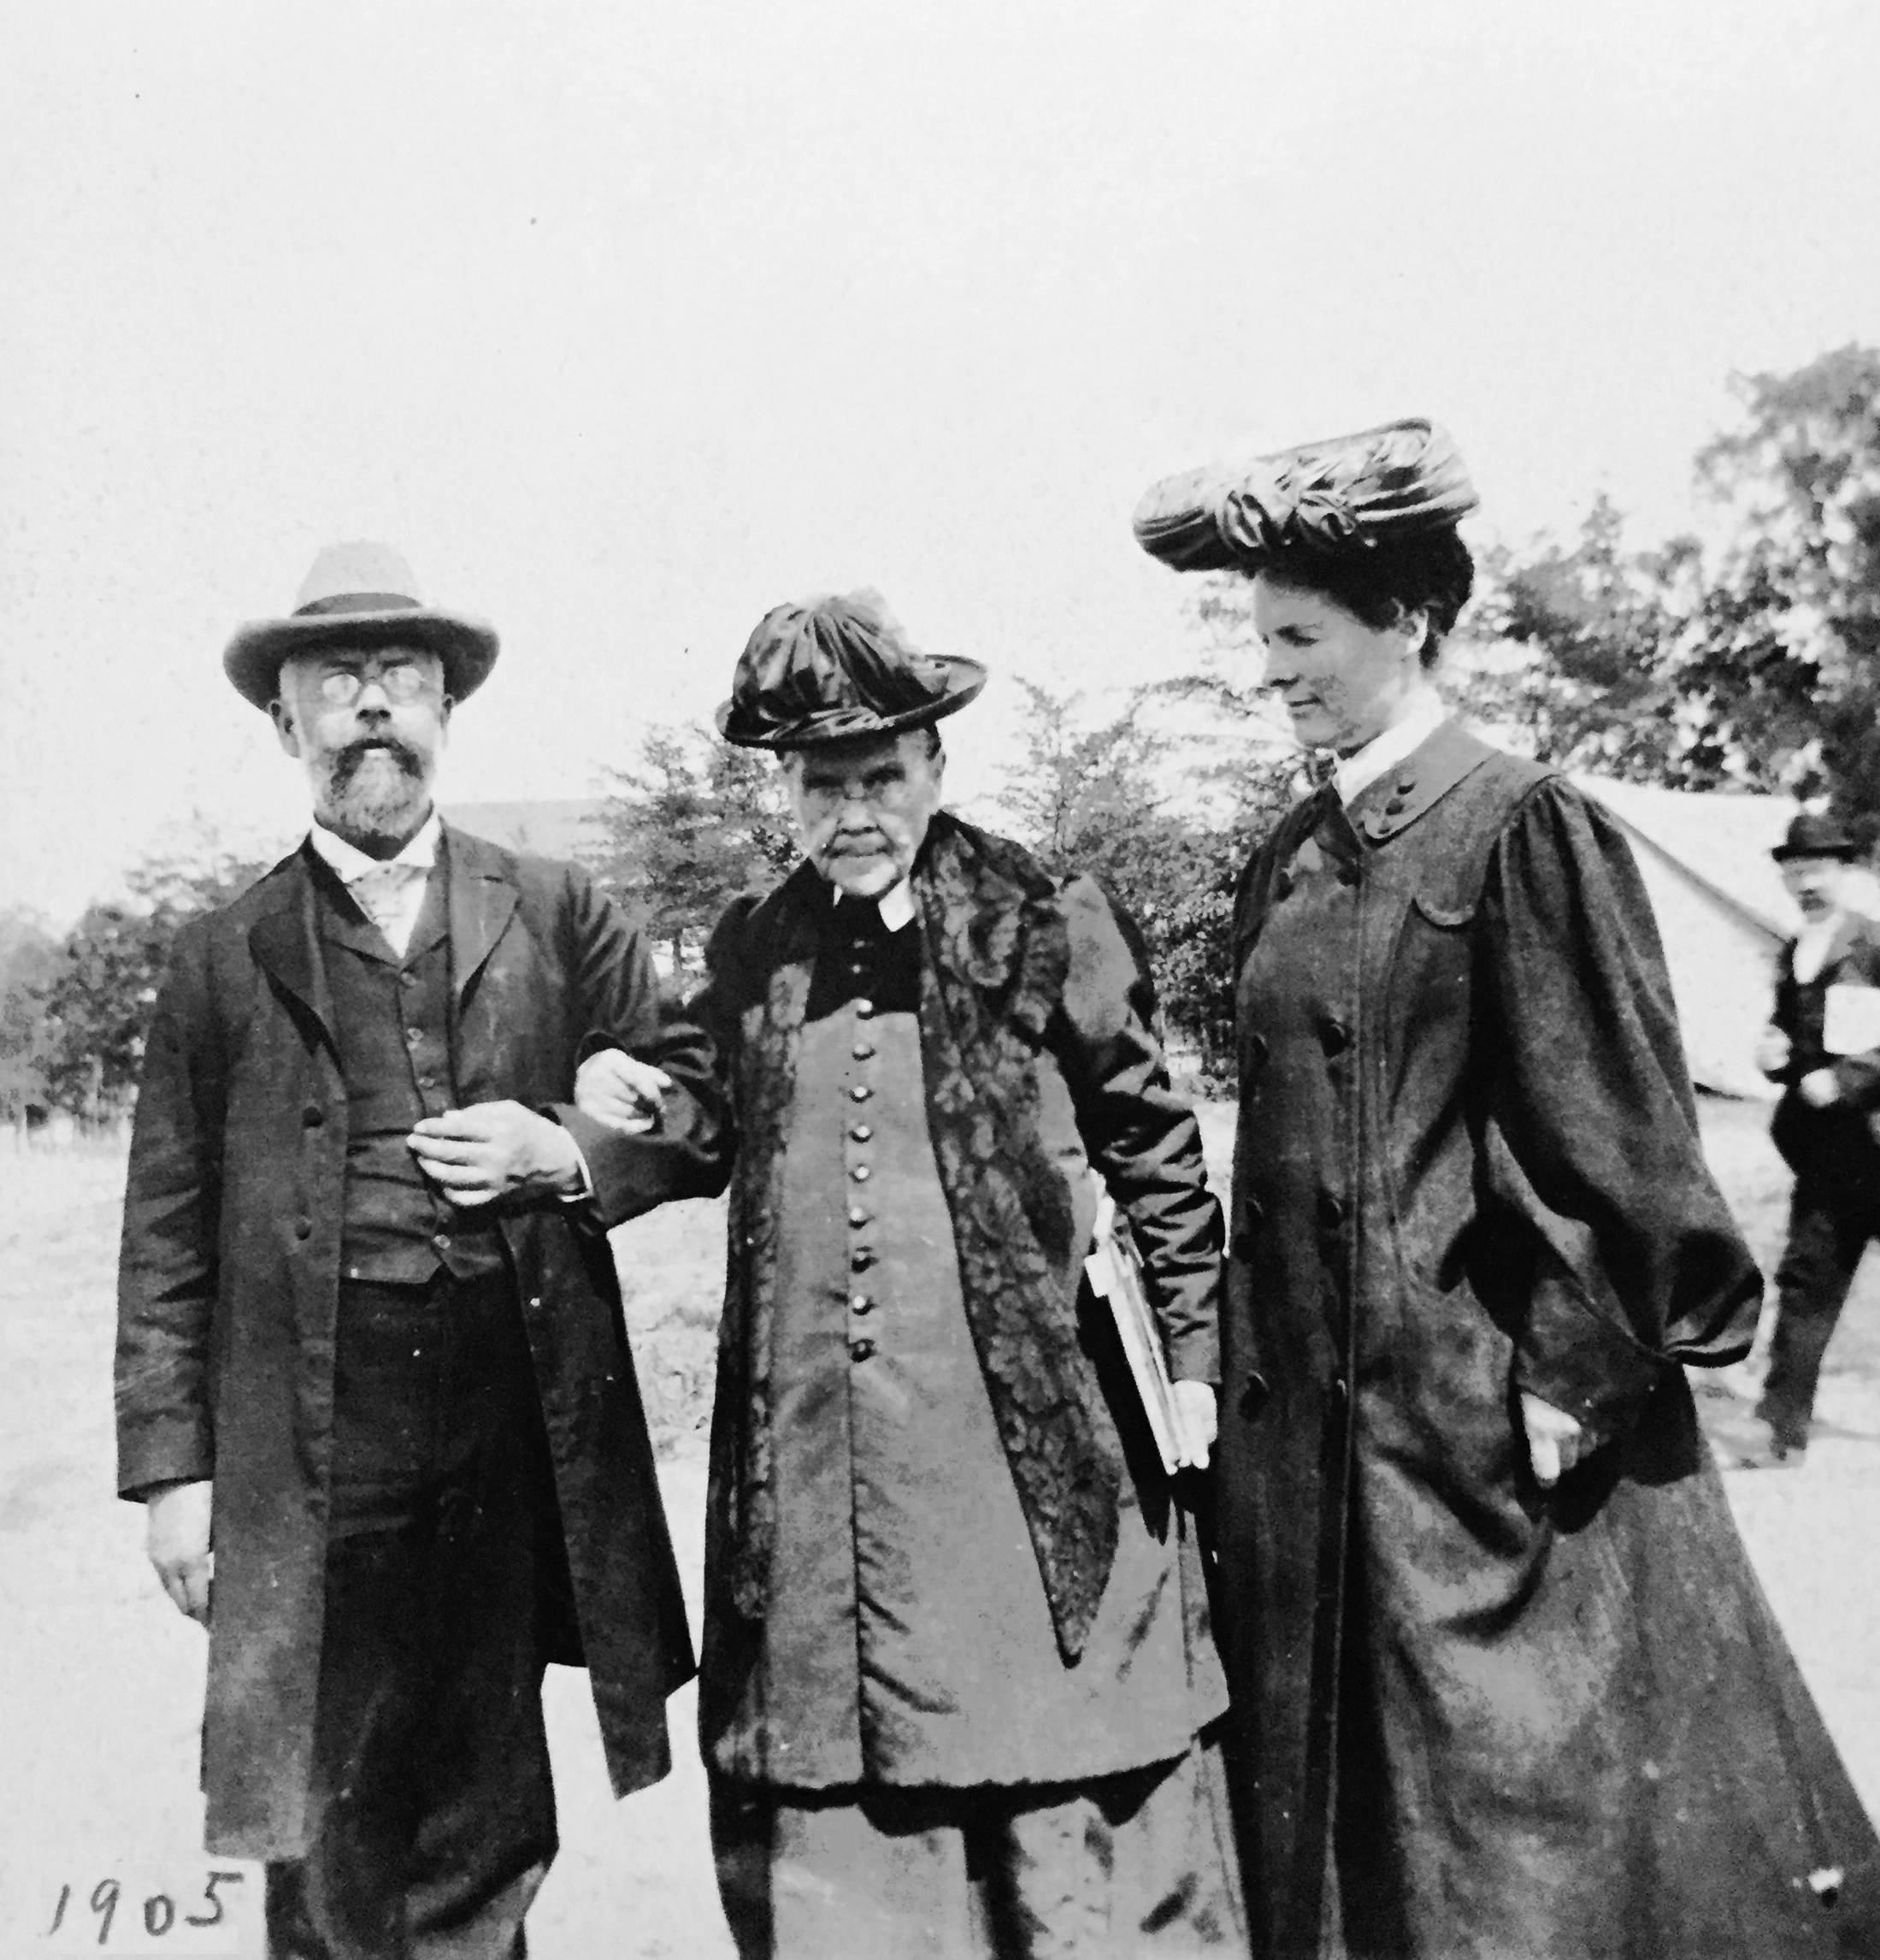
\includegraphics[width=1\linewidth]{images/william-ellen-white-1905.jpg}
    \caption*{William C. White i Ellen G. White, 1905}
    \label{fig:w-e-white}
\end{figure}

Prema Williamu Whiteu, naša jedina nada kao Adventista sedmog dana je pridržavanje prvobitnih principa. Ti principi, kako znamo, su \emcap{Fundamentalni Principi}. Zatim je spomenuo redoslijed kojim neprijatelj napada naš rad. Napad započinje našim nejedinstvom, zatim cilja na slabljenje našeg poštovanja prema Suboti i službi Svetišta, napada naše povjerenje u Duh Proroštva, i na kraju se fokusira na zbunjivanje naših koncepcija o osobnom Bogu.

Odgovor sestre White Williamu Whiteu je zapanjujuće prirode. Ona nam daje naslutiti da će se veliki otpad uskoro ostvariti i da je naša nada u pridržavanju prvobitnih principa naše vjere—\emcap{Fundamentalnih Principa}.

\egw{Elmshaven, St. Helena, Kalifornija} \\
\egw{4. prosinca 1905.} \\
\egw{W. C. White} \\
\egw{Moj dragi sine - }

\egw{...}

\egw{“\textbf{Jedna stvar je sigurna koja će se uskoro ostvariti—\underline{veliki otpad}, koji se razvija i povećava i osnažuje i \underline{nastavit će} tako sve dok Gospodin ne dođe s neba sa zvukom trube. \underline{Moramo se čvrsto držati prvih principa naše denominirane vjere} i krenuti naprijed iz snage do povećane vjere. \underline{Uvijek} moramo zadržati vjeru koju je potvrdio Božji Duh \underline{od najranijih događaja našeg iskustva do današnjeg vremena}.} Sada nam je potrebna šira širina i dublja, ozbiljnija, nepokolebljiva vjera u vodstvo Duha Svetoga. \textbf{Ako nam je u početku bio potreban očit dokaz o snazi Duha Svetoga koji je potvrdio istinu \underline{u početku}, nakon proteka vremena, \underline{tako su nam i danas potrebni svi dokazi u potvrdi istine}, kada duše odlaze od vjere, priklanjajući se prijevarnim duhovima i naucima zloduhā.} Ne smije biti malaksalosti duše sada. Ako je ikad postojalo razdoblje kada smo trebali snagu Duha Svetoga u našim govorima, u našim molitvama, u svakom predloženom djelu, to je sada. \textbf{Ne smijemo se zaustaviti na prvom iskustvu, ali dok nosimo \underline{istu poruku} ljudima, \underline{ova se poruka treba ojačati i proširiti}}. \textbf{Moramo vidjeti i razumjeti važnost poruke koja je učinjena sigurnom njenim božanskim podrijetlom}. Moramo nastaviti kako bismo upoznali Gospodina, da bismo mogli znati da je Njegov izlazak kao zora spreman. Naše duše trebaju osnaženje od Izvora svake moći. \textbf{Možemo se ojačati i utvrditi u našem prošlom iskustvu \underline{koje nas drži za bitne točke istine koja nas je učinila onim što jesmo—Adventisti Sedmoga Dana}.}”}[Lt326-1905.2; 1905][https://egwwritings.org/read?panels=p7678.8]

\egwnogap{\textbf{Posljednjih pedeset godina nije izblijedilo ni jednu jotu ili princip naše vjere kao što smo primili velike i čudesne dokaze koji su nam učinjeni sigurnim 1844, nakon proteka vremena.} Malaksale duše trebaju biti utvrđene i oživljene prema Njegovoj Riječi. Mnogi od propovjednika evanđelja i Gospodnjih liječnika naći će svoje malaksale duše oživljene prema Riječi. \textbf{\underline{Ni jedna riječ nije promijenjena ili poreknuta}.} \textbf{Ono za što je Duh Sveti svjedočio da je istina nakon proteka vremena, u našem velikom razočarenju, je \underline{čvrsti temelj istine}. Stupovi istine su bili otkriveni, i mi smo prihvatili \underline{temeljne principe} koji su nas učinili onim što jesmo—Adventisti Sedmog dana, držeći zapovijedi Božje i imajući vjeru Isusovu.}}[Lt326-1905.3; 1905][https://egwwritings.org/read?panels=p7678.9]

Ovo pismo je zapanjujuće jer je odgovor na redoslijed kako neprijatelj napada naš rad. Sestra White je dobro svjesna tih napada i predstavila je problem u pravom svjetlu, pokazujući nam također što trebamo učiniti kako bismo spriječili Sotonine napade na nas. Neprijatelj želi \others{zbuniti našu koncepciju o osobnom Bogu}. Ovo je upravo točka velikog otpadništva koje \egwinline{će se uskoro ostvariti}, i koje se \egwinline{povećava i osnažuje i nastavit će tako sve dok Gospodin ne dođe s neba sa zvukom trube}. Ovo je otpadništvo koje danas doživljavamo. Koja je naša nada protiv ove obmane i velikog otpadništva? \egwinline{\textbf{\underline{Moramo se čvrsto držati prvih principa naše denominirane vjere} i krenuti naprijed iz snage do povećane vjere. \underline{Uvijek} moramo zadržati vjeru koju je potvrdio Božji Duh od najranijih događaja našeg iskustva do današnjeg vremena.}} \egwinline{...\textbf{\underline{ova se poruka treba ojačati i proširiti}}...} \egwinline{...\textbf{\underline{danas su nam potrebni svi dokazi u potvrdi istine}}...} \egwinline{\textbf{Možemo se ojačati i utvrditi u našem prošlom iskustvu koje nas drži za bitne točke istine koja nas je učinila onim što jesmo—Adventisti Sedmoga Dana}}. Ove bitne točke istine, koje su nas učinile Adventistima Sedmog Dana, su \emcap{Fundamentalni Principi}, rođeni na početku našeg rada. Godine 1905. ona je napisala: \egwinline{\textbf{Posljednjih pedeset godina nije izblijedilo ni jednu jotu ili princip naše vjere kao što smo primili velike i čudesne dokaze koji su nam učinjeni sigurnim 1844, nakon proteka vremena.}} \egwinline{\textbf{Ni jedna riječ nije promijenjena ili poreknuta.} \textbf{Ono za što je Duh Sveti svjedočio da je istina nakon proteka vremena, u našem velikom razočarenju, je \underline{čvrsti temelj istine}. Stupovi istine su bili otkriveni, i mi smo prihvatili \underline{temeljne principe} koji su nas učinili onim što jesmo—Adventisti Sedmog dana, držeći zapovijedi Božje i imajući vjeru Isusovu.}}

Bog nas poziva da budemo postojani u \emcap{Fundamentalnim Principima}, posebno u vezi \others{koncepcije o osobnom Bogu}. Ovo je prva točka \emcap{Fundamentalnih Principa}.

Sestra White je prorekla da se u našoj crkvi razvija veliko otpadništvo u vezi s razumijevanjem \emcap{ličnosti Boga}. Ispravno razumijevanje \emcap{ličnosti Boga} prikazano je u \emcap{Fundamentalnim Principima}. Jasno nas je upozorila na Sotonin napad na ove principe. Poziva nas da se \egw{\textbf{čvrsto držati prvih principa naše denominirane vjere} i krenemo naprijed iz snage do povećane vjere}.

\egw{\textbf{“Nakon proteka vremena, Bog je svojim vjernim sljedbenicima povjerio dragocjene \underline{principe sadašnje istine}. Ti principi nisu dani onima koji nisu imali udjela u davanju poruke prvog i drugog anđela. Oni su dani radnicima koji su imali udjela u ovom djelu od samog početka}.”}[Ms129-1905.5; 1905][https://egwwritings.org/read?panels=p9797.12]

\egwnogap{\textbf{Oni koji su prošli kroz ta iskustva trebaju biti \underline{čvrsti kao stijena u principima} koji su nas učinili Adventistima Sedmog Dana}. Oni trebaju biti suradnici s Bogom, povezujući svjedočanstvo i pečateći zakon među Njegovim učenicima. Oni koji su sudjelovali u uspostavi našeg rada na temeljima biblijske istine; \textbf{oni koji znaju međaše koji su ukazivali na pravi put} trebaju se smatrati radnicima najviše vrijednosti. Oni mogu govoriti iz osobnog iskustva o istinama povjerenim njima. Ovi ljudi ne smiju dopustiti da se njihova vjera promijeni u nevjeru; ne smiju dopustiti da im se zastava trećeg anđela uzme iz ruku. Oni trebaju čvrsto držati početak svoje pouzdanosti do kraja. \textbf{\underline{Gospod je izjavio kako će se prošlost morati ponovno obnoviti kako ulazimo u završno djelo}. Svaka istina koju je On dao za ove posljednje dane ima biti objavljena svijetu. \underline{Svaki stup} koji je On utvrdio \underline{ima biti učvršćen}. Ne možemo sada sići sa temelja kojega je Bog učvrstio. Ne možemo sada ući u nikakvu novu organizaciju; jer to bi značilo otpadanje od istine}.}[Ms129-1905.6; 1905][https://egwwritings.org/read?panels=p9797.13]

Odstupanje od temelja koji je Bog uspostavio znači ulazak u novu organizaciju; to je otpadanje od istine. Uspoređujući \emcap{Fundamentalne Principe} iz prošlosti s trenutnim trinitarijanskim Temeljnim vjerovanjima, očito je da smo u stanju otpadništva. Ellen White je prorekla da će se ovaj otpad \egwinline{\textbf{koji se razvija i povećava i osnažuje i \underline{nastavit će} tako sve dok Gospodin ne dođe s neba sa zvukom trube}}[Lt326-1905.2; 1905][https://egwwritings.org/read?panels=p7678.8].

% The great apostasy is soon to be realized

\begin{titledpoem}
    \stanza{
        Proročanstvo Ellen White jasno zvoni, \\
        Otpad veliki uskoro se kruni; \\
        Držite se čvrsto prvih principa vjere, \\
        Dok se Sotonine zamke šire.
    }

    \stanza{
        Neprijatelj napada Božju istinu staru, \\
        Želi zbuniti našu o Bogu vjeru; \\
        Od temelja naših ne smijemo bježati, \\
        Već ih moramo snažno podržati.
    }

    \stanza{
        Pedeset godina nije izblijedilo ni jotu, \\
        Ni jednu riječ, ni jednu notu; \\
        Stupovi istine čvrsto stoje, \\
        Dok otpadništvo svoje mreže kroje.
    }
\end{titledpoem}

\begin{titledpoem}
    \stanza{
        Adventisti, čujte glas upozorenja, \\
        Dolazi vrijeme velikog iskušenja; \\
        Osobni Bog, prva točka naše vjere, \\
        Pod napadom je, dok se laži šire.
    }

    \stanza{
        "Suoči se!" zapovijed s neba stiže, \\
        Ellen White istinu visoko diže; \\
        Fundamentalni Principi su naša snaga, \\
        U njima je istina nama draga.
    }

    \stanza{
        Otpad raste i sve jači biva, \\
        Do Kristovog dolaska ne prestaje da se skriva; \\
        Držimo se čvrsto istine stare, \\
        Koja nas čini Adventistima prave vjere.
    }
\end{titledpoem}

\begin{titledpoem}
    \stanza{
        Temeljni principi, naše sidro u oluji, \\
        Dok se lažna učenja oko nas roji; \\
        Od 1844. istina stoji nepromijenjena, \\
        Duhom Svetim zauvijek potvrđena.
    }

    \stanza{
        Prošlost se mora obnoviti, Gospod kaže, \\
        Dok se kraj vremena pred nama slaže; \\
        Svaki stup mora biti učvršćen, \\
        Svaki temelj istine osnažen.
    }

    \stanza{
        Ne smijemo u novu organizaciju ući, \\
        To bi značilo od istine se odvući; \\
        Ostanimo vjerni principima prvim, \\
        I poruku istine svijetu objavimo svim.
    }
\end{titledpoem}